\apendice{Especificación de Requisitos}

\section{Introducción}

En este apéndice se recoge una descripción del sistema \emph{software} a desarrollar. Más concretamente, se presentan aspectos como el propósito, alcance y objetivos generales del mismo, así como los requisitos específicos que el sistema debe implementar.

La forma en la que hemos organizado la Especificación está basada parcialmente en las recomendaciones del estándar IEEE 830-1998, considerado como la principal referencia para la aplicación de buenas prácticas en la escritura del Documento de Especificación de Requistios (SRS).

\subsection{Propósito}

El propósito de la presente Especificación de Requisitos tiene como objetivo ofrecer una descripción detallada del sistema \emph{software} desarrollado.

Este documento está orientado principalmente al equipo de desarrollo del proyecto, pero queda también a libre disposición de cualquier persona que pudiera estar interesada.

\subsection{Alcance}

El sistema \emph{software} a desarrollar recibirá el nombre de JIZT. El objetivo y funcionalidad principal de JIZT será la generación de resúmenes abstractivos en la nube. Dicho sistema estará orientado tanto a usuarios con conocimientos de informática básicos, así como usuarios con experiencia en el campo.

Para los primeros, es decir, usuarios con conocimientos básicos, se ofrecerá una aplicación multiplataforma desarrollada con la usabilidad en mente.

Para aquellos usuarios más avanzados, además de la aplicación, se proporcionará una API REST, permitiéndoles realizar peticiones directamente, e incluso desarrollar sus propias aplicaciones que consuman dicha API.

Se pondrá especial atención en el desarrollo de una documentación completa, accesible y de fácil comprensión. Esta documentación recogerá tanto los aspectos técnicos de la aplicación y la API REST, así como manuales de uso para el usuario y para el desarrollador.

\subsection{Definiciones, siglas, y abreviaciones}

A continuación se recogen las definiciones, siglas y abreviaciones más relevantes para el proyecto:

\vspace{-0.3cm}
\begin{itemize} [\textbullet]
	\item \textbf{NLP}: Procesamiento de Lenguaje Natural (\emph{Natural Language Processing}).
	\vspace{-0.1cm}
	\item \textbf{Resumen extractivo}: aquel resumen generado a partir de la \emph{extracción} de las frases del texto consideradas más relevantes. Es decir, este tipo de resúmenes contienen únicamente frases tomadas literalmente del texto original.
	\vspace{-0.1cm}
	\item \textbf{Resumen abstractivo}: aquel resumen que incluye palabras o expresiones que no aparecen en el texto original.
	\vspace{-0.1cm}
	\item \textbf{API REST}: servicio \emph{web} que proporciona una serie de \emph{endpoints} para llevar a cabo operaciones HTTP (métodos), que proporcionan acceso para crear, recuperar, actualizar o eliminar los recursos del servicio.
	\vspace{-0.1cm}
	\item \textbf{\emph{Endpoint}}: punto de entrada en un canal de comunicación cuando dos sistemas interactúan. En una API REST los \emph{endpoints} son generalmente URLs.
	\vspace{-0.1cm}
	\item \textbf{HTTP}: \emph{Hypertext Transfer Protocol}, protocolo para sistemas de información distribuidos, colaborativos e hipermedia. Este protocolo es la base de la comunicación de datos para la World Wide Web (WWW).
	\vspace{-0.1cm}
	\item \textbf{URL}: \emph{Uniform Resource Locator}, referencia a un recurso web que especifica su ubicación en una red informática y un mecanismo para recuperarlo.
	\vspace{-0.1cm}
	\item \textbf{\emph{Frontend}}: la infraestructura \emph{frontend} incluye todos aquellos elementos del sistema con los que el usuario final interactúa.
	\vspace{-0.1cm}
	\item \textbf{\emph{Backend}}:parte de la infraestructura que contiene el conjunto de servidores, bases de datos, APIs y los sistemas operativos que alimentan el \emph{frontend} de una aplicación.
\end{itemize}

\section{Descripción global}

\subsection{Objetivos generales}

Los principales objetivos del sistema \emph{software} a desarrollar son los siguientes:

\vspace{-0.3cm}
\begin{itemize} [\textbullet]
	\item Implementar un servicio de generación de resúmenes abstractivos en la nube, empleando modelos pre-entrenados del estado del arte.
	\vspace{-0.1cm}
	\item Implementar el \emph{backend} que haga posible esta generación de resúmenes, así como una API REST para exponer el \emph{backend}.
	\vspace{-0.1cm}
	\item Diseñar la arquitectura del \emph{backend} con aspectos como la flexibilidad, la escalabilidad y la alta disponibilidad como pilares fundamentales.
	\vspace{-0.1cm}
	\item Implementar un \emph{frontend} (aplicación multiplataforma) que consuma la REST API y dé la posibilidad de generar resúmenes a cualquier usuario.
	\vspace{-0.1cm}
	\item Implementar una interfaz (tanto en el \emph{backend} como en el \emph{fontend}) que permita a los usuarios especificar los parámetros con los que el resumen será generado, como por ejemplo, su longitud relativa al texto original.
	
\end{itemize}


\subsection{Características del usuario}

Los usuarios potenciales de JIZT se pueden dividir en dos categorías fundamentales:

\vspace{-0.3cm}
\begin{itemize} [\textbullet]
	\item Estudiantes de edades comprendidas entre los 15 y 25 años. El uso principal que harán del producto será el resumen de textos académicos.
	\item Personas de edades comprendidas entre los 25 y 50 años, cuyo principal uso será el resumen de noticias y artículos periodísticos.
\end{itemize}

En cuanto al sexo, el uso por parte tanto de hombres como mujeres será aproximadamente equivalente.

Un tercer tipo de usuario, no incluido anteriormente, serían partidos interesados en el uso del producto, como empresas o particulares, que fueran a hacer un uso extensivo y exhaustivo del mismo. Este tipo de usuario requiere unas prestaciones más exigentes, pudiendo llegar a solicitar el despliegue de JIZT en sus propias dependencias.

Es por ello que el producto desarrollado deberá ser lo más independiente del entorno en el que se despliegue como sea posible.


\section{Catalogo de requisitos}

A continuación se detallan los requisitos funcionales y no funcionales del producto a desarrollar. Estos requisitos son globales al proyecto y, por tanto, involucran tanto al \emph{backend} como a la aplicación a desarrollar.

\subsection{Requisitos funcionales}

\begin{itemize}[\textbullet]
	\item \textbf{RF-1 Solicitar resumen}: la API REST debe proporcionar un \emph{endpoint} para que el usuario pueda solicitar un resumen de un texto.
	\begin{itemize}[◦]
		\item \textbf{RF-1.1 Elegir modelo de generación de resumen}: el usuario deberá ser capaz de especificar el modelo de generar su resumen\footnote{\, Este requisito solo se ha implementado en el \emph{backend}. En la aplicación decidimos no incluirlo dado que por el momento solo hacemos uso de un modelo.}.
		\item \textbf{RF-1.2 Especificar longitud relativa del resumen}: el usuario deberá ser capaz de especificar la longitud del resumen generado, de manera relativa al texto original.
		\item \textbf{RF-1.3 Especificar parámetros del resumen}: el usuario deberá ser capaz de especificar los parámetros concretos con los que se generará su resumen\footnote{\, Este requisito solo se ha implementado en el \emph{backend}. En la aplicación se añadirá en futuras iteraciones, al considerarse no prioritario, dado que se trata de opciones avanzadas.}.
	\end{itemize}
	\item \textbf{RF-2 Historial de resúmenes}: el usuario podrá acceder a los resúmenes que ha generado recientemente.
	\item \textbf{RF-3 Compartir resumen}: se le brindará al usuario la opción de compartir el resumen generado a través de otra aplicación a su elección.
	\item \textbf{RF-4 Copiar resumen}: se le brindará al usuario la opción de copiar el resumen generado.
	\item \textbf{RF-5 Borrar resumen}: el usuario deberá ser capaz de borrar permanentemente un resumen previamente generado.
	\item \textbf{RF-6 Pegar desde el portapapeles}: la aplicación ofrecerá una opción para que el usuario pueda pegar el texto a resumir desde el portapapeles de forma sencilla.
	\item \textbf{RF-7 Mostrar metadatos}: el sistema brindará al usuario los metadatos relativos al resumen generado, como la hora a la que fue creado.
	\item \textbf{RF-8 Pre-procesado del texto}: el sistema será capaz de recibir texto con errores de formateo (exceso de espacios, saltos de carro situados en mitad de una frase, etc.), así como caracteres <<extraños>>. Independientemente de lo anterior, el resumen generado aparecerá correctamente formateado y sin los mencionados caracteres.
	\item \textbf{RF-9 Textos arbitrariamente largos}: el sistema será capaz de producir resúmenes de cualquier texto, independientemente de la longitud de los mismos. No se espera, no obstante, que el tiempo de resumen de textos extremadamente largos esté por debajo del orden del minuto.
\end{itemize}

\subsection{Requisitos no funcionales}

\begin{itemize}[\textbullet]
	\item \textbf{RNF-1 Escalabilidad}: la arquitectura del sistema deberá permitir el escalado del mismo de forma rápida y sencilla.
	\begin{itemize}[◦]
		\item \textbf{RNF-1.1 Autoescalado}: el sistema podrá escalarse de manera automática en momentos en los que la carga de trabajo así lo requiera. Del mismo modo, cuando dicha carga remita, deberá disminuir su escala, a fin de consumir los mínimos recursos posibles.
	\end{itemize}
	\item \textbf{RNF-2 Alta disponibilidad}: el sistema deberá garantizar el acceso al mismo por parte de los usuarios en el 99,99 \% de los casos.
	\begin{itemize}[◦]
		\item \textbf{RNF-2.1 Tolerancia frente a fallos}: el sistema deberá ser capaz de recuperarse de forma automática de posibles errores o problemas de funcionamiento de cualquiera de sus componentes en un tiempo menor a los 2 minutos.
	\end{itemize}
	\item \textbf{RNF-3 Eficiencia}: el sistema deberá ser capaz de generar un elevado número de resúmenes provenientes de diferentes usuarios de forma simultánea, sin que el tiempo medio de resumen se vea afectado.
	\item \textbf{RNF-4 Seguridad lógica y de datos}: se debe garantizar la correcta protección de todos los datos manejados por el sistema.
	\item \textbf{RNF-5 Privacidad}: se debe asegurar la protección de los datos de carácter personal.
	\begin{itemize}[◦]
		\item \textbf{RNF-5.1 Anonimidad}: en ningún caso se recopilará información de los usuarios que permita determinar la identidad de los mismos. No obstante, el sistema no es responsable de garantizar que los textos introducidos no contienen información de carácter personal.
	\end{itemize}
	\item \textbf{RNF-6 Usabilidad}: el tiempo medio de aprendizaje de la aplicación por parte de los usuarios deberá ser inferior a los 5 minutos. Además, el sistema contará con documentación en línea detallada del producto.
	\item \textbf{RNF-7 Multiplataforma}: se distribuirán los binarios de la aplicación necesarios para su ejecución en móvil (Android e iOS), \emph{web} (Google Chrome, Mozilla Firefox, Safari y Microsoft Edge), y escritorio (Linux, Apple y Windows).
	\item \textbf{RNF-8 Tamaño reducido}: el peso de la aplicación no debe superar los 30 MB.
\end{itemize}

\newpage

\section{Especificación de requisitos}

En esta sección, nos centramos en la definición de los casos de uso de nuestro producto.

Dado que el usuario interactuará únicamente con la aplicación (\emph{frontend}), el \emph{backend} no se considera en este caso, aunque sigue siendo vital para que los casos de uso de la aplicación se puedan completar con éxito.

\subsection{Diagrama de casos de uso}



\begin{figure}[h!]
	\centering
	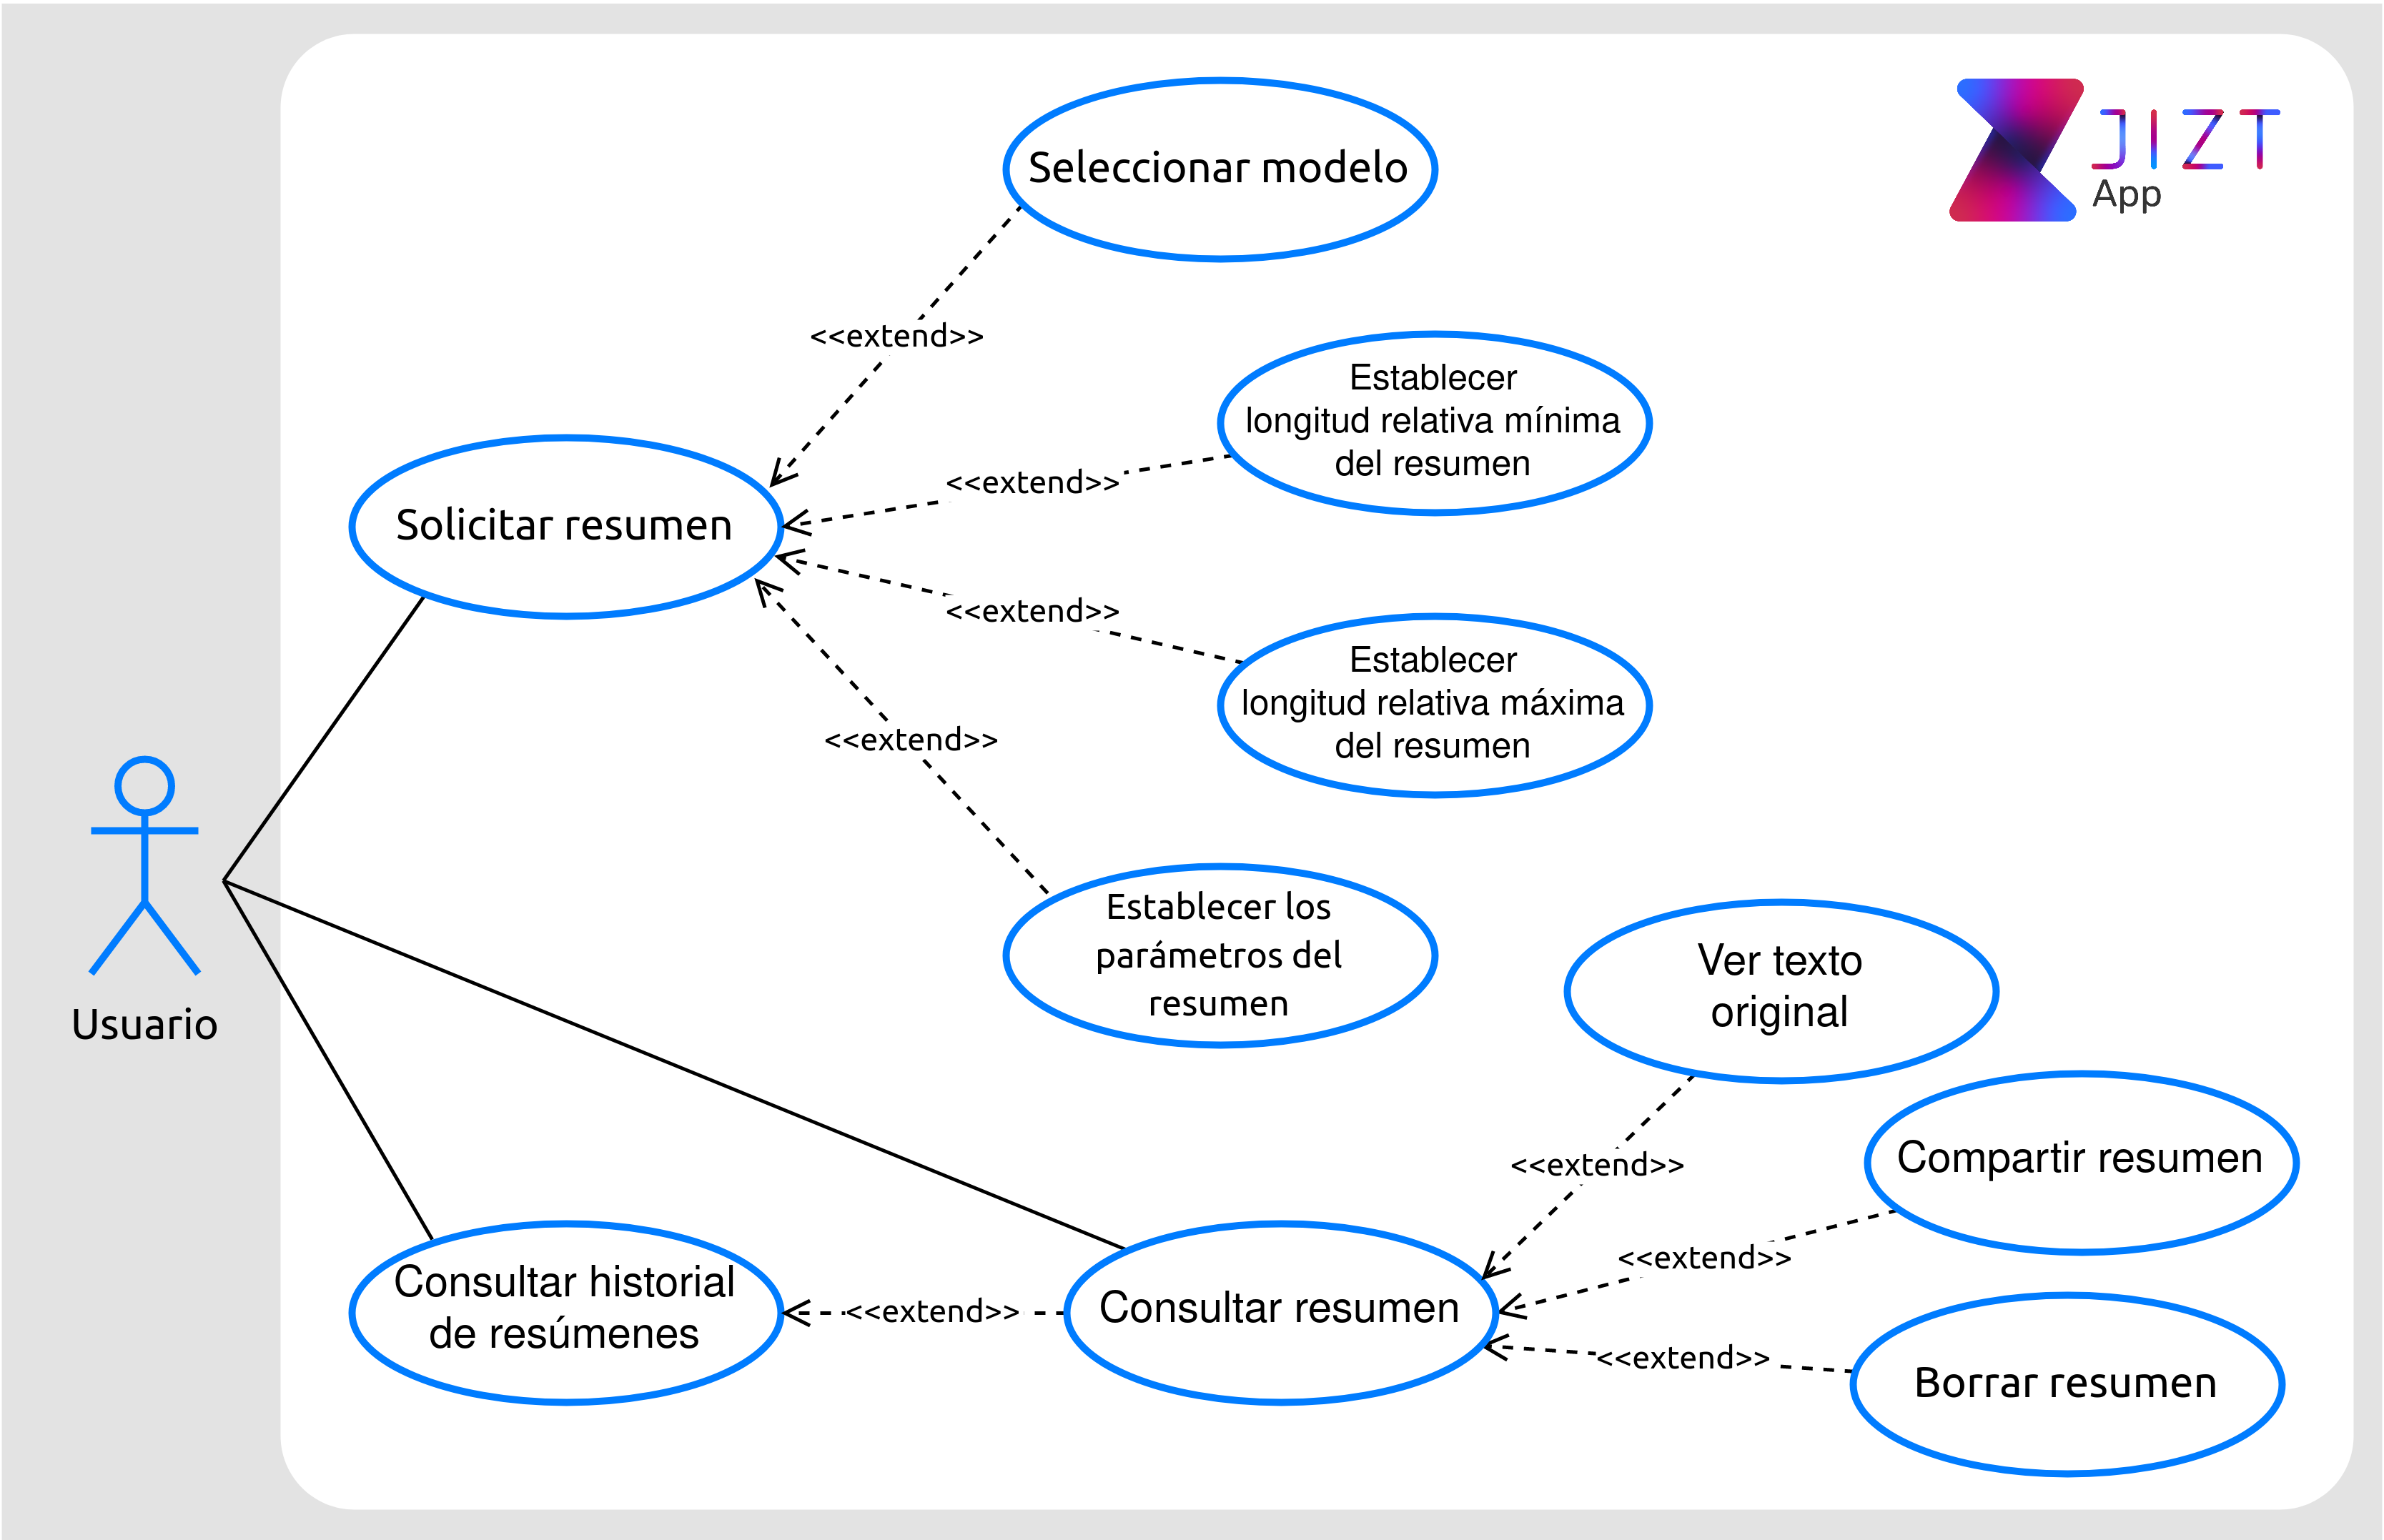
\includegraphics[width=\textwidth]{use-case-diagram}
	\vspace{-0.5cm}
	\caption{Diagrama de casos de uso.}
	\label{flutter-widgets}
\end{figure}

\subsection{Actores}

Existe un único actor: el usuario que hace uso de la aplicación.


\subsection{Casos de uso}

\begin{longtable}{>{\raggedright}b{0.2\linewidth}>{\raggedright\arraybackslash}b{0.7\linewidth}}
	\toprule
	\textbf{CU-01} & \textbf{Solicitar resumen} \\
	\toprule
	\endhead

	\toprule
	\caption{CU-01 Solicitar resumen}
	\endfoot
	
	\small{\textbf{Descripción}} & Solicitar la generación de un resumen a partir de un \\
	& texto. \\
	\small{\textbf{Autor}} & Diego Miguel Lozano \\
	\small{\textbf{Requisitos}} & RF-1, RF-6, RF-8, RF-9 \\
	\small{\textbf{relacionados}} & \\
	\small{\textbf{Precondición}} & La API REST se encuentra accesible. \\
	\small{\textbf{Flujo normal}} & \quad {\small 1. El usuario inicia la aplicación.} \\
	& \quad {\small 2. El usuario hace \emph{click} en} \\
	& \qquad {\small el área de texto.} \\
	& \quad {\small 3. El usuario introduce el texto a resumir o, alterna-} \\
	& \qquad {\small tivamente, lo pega desde el portapapeles.} \\
	& \quad {\small 4. El usuario pulsa en el botón <<\emph{Summarize}>>.} \\
	& \quad {\small 5. Se muestra un indicador de <<procesando>>.} \\
	& \quad {\small 6. Se muestra un indicador de <<resumen completado>>.} \\
	& \quad {\small 7. Se muestra el resumen generado.} \\
	\small{\textbf{Postcondición}} & El usuario ha obtenido el resumen de su texto. \\
	\small{\textbf{Excepciones}} & API REST inaccesible. \\
	\small{\textbf{Incluye}} & - \\
	\small{\textbf{Extiende}} & - \\
	\small{\textbf{Prioridad}} & Muy alta. \\
	\small{\textbf{Frecuencia de}} & Muy alta. \\
	\small{\textbf{uso}} & \\
	\small{\textbf{Importancia}} & Crítica. \\
	\small{\textbf{Comentarios}} & - \\
\end{longtable}


\begin{longtable}{>{\raggedright}b{0.2\linewidth}>{\raggedright\arraybackslash}b{0.7\linewidth}}
	\toprule
	\textbf{CU-02} & \textbf{Establecer longitud relativa mínima del resumen} \\
	\toprule
	\endhead
	
	\toprule
	\caption{CU-02 Establecer longitud relativa mínima del resumen}
	\endfoot
	
	\small{\textbf{Descripción}} & Establecer la longitud mínima que puede tener el \\
	& resumen generado de manera relativa al texto \\ & original. \\
	\small{\textbf{Autor}} & Diego Miguel Lozano \\
	\small{\textbf{Requisitos}} & RF-1.2  \\
	\small{\textbf{relacionados}} & \\
	\small{\textbf{Precondición}} & - \\
	\small{\textbf{Flujo normal}} & \quad \small{1. El usuario pulsa sobre el cuadro de texto en la} \\
	& \qquad \small{pantalla principal.} \\
	& \quad \small{2. El usuario ajusta la longitud mínima a través del} \\
	& \qquad \small{\emph{slider} que aparece en la parte inferior de la pantalla} \\
	\small{\textbf{Postcondición}} & Se ha establecido la longitud mínima. \\
	\small{\textbf{Excepciones}} & - \\
	\small{\textbf{Incluye}} & - \\
	\small{\textbf{Extiende}} & - \\
	\small{\textbf{Prioridad}} & Alta. \\
	\small{\textbf{Frecuencia de}} & Alta. \\
	\small{\textbf{uso}} & \\
	\small{\textbf{Importancia}} & Alta. \\
	\small{\textbf{Comentarios}} &  - \\
\end{longtable}

\begin{longtable}{>{\raggedright}b{0.2\linewidth}>{\raggedright\arraybackslash}b{0.7\linewidth}}
	\toprule
	\textbf{CU-03} & \textbf{Establecer longitud relativa máxima del resumen} \\
	\toprule
	\endhead
	
	\toprule
	\caption{CU-03 Establecer longitud relativa máxima del resumen}
	\endfoot
	
	\small{\textbf{Descripción}} & Establecer la longitud máxima que puede tener el \\
	& resumen generado de manera relativa al texto \\ & original. \\
	\small{\textbf{Autor}} & Diego Miguel Lozano \\
	\small{\textbf{Requisitos}} & RF-1.2  \\
	\small{\textbf{relacionados}} & \\
	\small{\textbf{Precondición}} & - \\
	\small{\textbf{Flujo normal}} & \quad \small{1. El usuario pulsa sobre el cuadro de texto en la} \\
	& \qquad \small{pantalla principal.} \\
	& \quad \small{2. El usuario ajusta la longitud máxima a través del} \\
	& \qquad \small{\emph{slider} que aparece en la parte inferior de la pantalla} \\
	\small{\textbf{Postcondición}} & Se ha establecido la longitud máxima. \\
	\small{\textbf{Excepciones}} & - \\
	\small{\textbf{Incluye}} & - \\
	\small{\textbf{Extiende}} & - \\
	\small{\textbf{Prioridad}} & Alta. \\
	\small{\textbf{Frecuencia de}} & Alta. \\
	\small{\textbf{uso}} & \\
	\small{\textbf{Importancia}} & Alta. \\
	\small{\textbf{Comentarios}} &  - \\
\end{longtable}



\begin{longtable}{>{\raggedright}b{0.2\linewidth}>{\raggedright\arraybackslash}b{0.7\linewidth}}
	\toprule
	\textbf{CU-04} & \textbf{Consultar historial de resúmenes} \\
	\toprule
	\endhead
	
	\toprule
	\caption{CU-04 Consultar historial de resúmenes}
	\endfoot
	
	\small{\textbf{Descripción}} & Visualizar la lista de resúmenes generados previa- \\
	& mente. \\
	\small{\textbf{Autor}} & Diego Miguel Lozano \\
	\small{\textbf{Requisitos}} & RF-2, RF-3, RF-4, RF-5, RF-7  \\
	\small{\textbf{relacionados}} & \\
	\small{\textbf{Precondición}} & Haber generado al menos un resumen previamente. \\
	\small{\textbf{Flujo normal}} & \quad \small{1. El usuario pulsa en <<\emph{See all}>> en la pantalla princi-} \\
	& \qquad \small{pal.} \\
	& \quad \small{2. Se muestra la lista de resúmenes previos.} \\
	\small{\textbf{Postcondición}} & Se visualizan los resúmenes generados. \\
	\small{\textbf{Excepciones}} & - \\
	\small{\textbf{Incluye}} & - \\
	\small{\textbf{Extiende}} & CU-07 \\
	\small{\textbf{Prioridad}} & Alta. \\
	\small{\textbf{Frecuencia de}} & Alta. \\
	\small{\textbf{uso}} & \\
	\small{\textbf{Importancia}} & Alta. \\
	\small{\textbf{Comentarios}} & Si aún no se ha generado ningún resumen, la lista\\
	& se mostrará vacía. \\
\end{longtable}


\begin{longtable}{>{\raggedright}b{0.2\linewidth}>{\raggedright\arraybackslash}b{0.7\linewidth}}
	\toprule
	\textbf{CU-05} & \textbf{Consultar resumen} \\
	\toprule
	\endhead
	
	\toprule
	\caption{CU-05 Consultar resumen}
	\endfoot
	
	\small{\textbf{Descripción}} & Consultar un resumen generado previamente. \\
	\small{\textbf{Autor}} & Diego Miguel Lozano \\
	\small{\textbf{Requisitos}} & RF-2  \\
	\small{\textbf{relacionados}} & \\
	\small{\textbf{Precondición}} &  Haber generado al menos un resumen previamente. \\
	\small{\textbf{Flujo normal}} & \small{Flujo 1:} \\
	& \quad \small{1. El usuario pulsa en uno de los resúmenes que apa-} \\
	& \qquad \small{recen en el inferior de la pantalla.} \\
	& \small{Flujo 2 (altenativa):} \\
	& \quad \small{1. El usuario pulsa en <<\emph{See all}>> en la pantalla prin-} \\
	& \qquad \small{cipal.} \\
	& \quad \small{2. Se muestra la lista de resúmenes previos.} \\
	& \quad \small{3. El usuario pulsa en uno de los resúmenes.} \\
	\small{\textbf{Postcondición}} & Se ha mostrado el resumen seleccionado. \\
	\small{\textbf{Excepciones}} & - \\
	\small{\textbf{Incluye}} & -\\
	\small{\textbf{Extiende}} & CU-06 \\
	\small{\textbf{Prioridad}} & Muy alta. \\
	\small{\textbf{Frecuencia de}} & \\
	\small{\textbf{uso}} & Alta. \\
	\small{\textbf{Importancia}} & Crítica. \\
	\small{\textbf{Comentarios}} & - \\
\end{longtable}


\begin{longtable}{>{\raggedright}b{0.2\linewidth}>{\raggedright\arraybackslash}b{0.7\linewidth}}
	\toprule
	\textbf{CU-06} & \textbf{Ver texto original} \\
	\toprule
	\endhead
	
	\toprule
	\caption{CU-06 Ver texto original}
	\endfoot
	
	\small{\textbf{Descripción}} & Visualizar el texto a partir del cual se ha generado \\
	& el resumen. \\
	\small{\textbf{Autor}} & Diego Miguel Lozano \\
	\small{\textbf{Requisitos}} & RF-2, RF-7  \\
	\small{\textbf{relacionados}} & \\
	\small{\textbf{Precondición}} & Haber generado un resumen. \\
	\small{\textbf{Flujo normal}} & \quad \small{1. El usuario pulsa en <<\emph{Original}>>. } \\
	\small{\textbf{Postcondición}} & Se ha mostrado el texto original.\\
	\small{\textbf{Excepciones}} & - \\
	\small{\textbf{Incluye}} & - \\
	\small{\textbf{Extiende}} & CU-07 \\
	\small{\textbf{Prioridad}} & Alta. \\
	\small{\textbf{Frecuencia de}} & Alta. \\
	\small{\textbf{uso}} & \\
	\small{\textbf{Importancia}} & Crítica. \\
	\small{\textbf{Comentarios}} & - \\
\end{longtable}


\begin{longtable}{>{\raggedright}b{0.2\linewidth}>{\raggedright\arraybackslash}b{0.7\linewidth}}
	\toprule
	\textbf{CU-07} & \textbf{Compartir el resumen} \\
	\toprule
	\endhead
	
	\toprule
	\caption{CU-07 Compartir el resumen}
	\endfoot
	
	\small{\textbf{Descripción}} & Compartir el resumen generado a través de otra \\
	& aplicación. \\
	\small{\textbf{Autor}} & Diego Miguel Lozano \\
	\small{\textbf{Requisitos}} & RF-3  \\
	\small{\textbf{relacionados}} & \\
	\small{\textbf{Precondición}} & Haber generado un resumen. \\
	\small{\textbf{Flujo normal}} & \quad \small{1. El usuario pulsa en el icono de compartir.} \\
	& \quad \small{2. Se muestra una lista de aplicaciones.} \\
	& \quad \small{3. El usuario pulsa en la aplicación a través de la cual} \\
	& \qquad \small{quiere compartir el resumen} \\
	\small{\textbf{Postcondición}} & Se ha compartido el resumen. \\
	\small{\textbf{Excepciones}} & - \\
	\small{\textbf{Incluye}} & - \\
	\small{\textbf{Extiende}} & CU-07 \\
	\small{\textbf{Prioridad}} & Media. \\
	\small{\textbf{Frecuencia de}} & Media. \\
	\small{\textbf{uso}} & \\
	\small{\textbf{Importancia}} & Media. \\
	\small{\textbf{Comentarios}} & - \\
\end{longtable}


\begin{longtable}{>{\raggedright}b{0.2\linewidth}>{\raggedright\arraybackslash}b{0.7\linewidth}}
	\toprule
	\textbf{CU-08} & \textbf{Borrar el resumen} \\
	\toprule
	\endhead
	
	\toprule
	\caption{CU-08 Borrar el resumen}
	\endfoot
	
	\small{\textbf{Descripción}} & Borrar un resumen generado. \\
	\small{\textbf{Autor}} & Diego Miguel Lozano \\
	\small{\textbf{Requisitos}} & RF-5  \\
	\small{\textbf{relacionados}} & \\
	\small{\textbf{Precondición}} & Haber generado un resumen. \\
	\small{\textbf{Flujo normal}} & \quad \small{1. El usuario pulsa en el icono de borrar.} \\
	 & \quad \small{2. Se elimina el resumen y la aplicación vuelve a} \\
	 & \qquad \small{la pantalla principal.} \\
	\small{\textbf{Postcondición}} & Se ha borrado el resumen. \\
	\small{\textbf{Excepciones}} & - \\
	\small{\textbf{Incluye}} & - \\
	\small{\textbf{Extiende}} & CU-07 \\
	\small{\textbf{Prioridad}} & Alta. \\
	\small{\textbf{Frecuencia de}} & Baja. \\
	\small{\textbf{uso}} & \\
	\small{\textbf{Importancia}} & Alta. \\
	\small{\textbf{Comentarios}} & - \\
\end{longtable}